\documentclass[a4paper,12pt]{scrartcl}
\usepackage{setspace}
\usepackage[utf8x]{inputenc}
\usepackage{ngerman}
\usepackage{graphicx}
\usepackage{enumerate}
\usepackage[font=small,labelfont=bf,singlelinecheck=false]{caption}
\usepackage[headsepline,plainheadsepline]{scrpage2}
\pagestyle{scrheadings}
\ohead[]{Christian Casar, Maximilian Menzel}
\ihead{HR - Blatt 4}



\begin{document}
\parindent0mm
\setcapindent{0pt}
\subsubsection*{Parallelisierung mit OpenMP}
\begin{table}
\begin{tabular}{|l|r|r|r|r|}
\hline
Implementation&1. Messung&2. Messung&3. Messung&Mittel\\
\hline
sequentiell&	1146,8643&	1146,7031&	1146,5567&	1146,7080\\
\hline
OpenMP	&137,0301	&122,0230	&121,7702&	126,9411\\
\hline
\end{tabular}
\caption{\textbf{Laufzeitmessung der verschiedenen Implementationen.}\\ 12 Threads, 512 Interlines, 1024 Iterationen, Messwerte jeweils in Sekunden}
\end{table}
\subsubsection*{Umsetzung der Datenaufteilung}
\begin{table}[!h]
\begin{tabular}{|l|r|r|r|r|r|}
\hline
Aufteilung&1. Messung&2. Messung&3. Messung&Mittel\\
\hline
Spalten	&462,5158	&462,0107	&469,3247	&464,6171\\
\hline
Zeilen	&265,1645	&264,5286	&263,9908	&264,5613\\
\hline
Elemente	&307,6507	&306,1153	&307,3371	&307,0344\\
\hline
\end{tabular}
\caption{\textbf{Laufzeitmesung der verschiedenen Datenaufteilungen.}\\ 12 Threads, 1024 Interlines, 512 Iterationen, Messwerte jeweils in Sekunden}
\end{table}

\subsubsection*{Vergleich der OpenMP-Scheduling-Algorithmen}

\begin{table}[!h]
\begin{tabular}{|l|r|r|r|r|r|}
\hline
Aufteilung&1. Messung&2. Messung&3. Messung&Mittel\\
\hline
static, 1&	303,3490&	304,5333&	304,8386&	304,2403\\
\hline
static, 2	&274,9212	&277,7070	&298,0135	&283,5472\\
\hline
static, 4	&632,1384	&632,3892	&633,6942	&632,7406\\
\hline
static, 16	&321,0543	&321,5812	&323,5345	&322,0567\\
\hline
dynamic, 1	&318,6475	&320,6304	&321,2673	&320,1818\\
\hline
dyamic, 4	&321,1643	&322,1790	&322,5387	&321,9607\\
\hline
guided	&321,0404	&321,3633	&322,7657	&321,7231\\

\hline
\end{tabular}
\caption{\textbf{Laufzeitmessung der Scheduling-Algorithmen für \\elementeweise Datenaufteilung.} 12 Threads, 1024 Interlines, 512 \\Iterationen, Messwerte jeweils in Sekunden}
\end{table}

\begin{table}[!h]
\begin{tabular}{|l|r|r|r|r|r|}
\hline
Aufteilung&1. Messung&2. Messung&3. Messung&Mittel\\
\hline
sta1s	&428,6237	&429,0607	&437,0074	&431,5639\\
\hline
static, 2	&426,8766	&429,3899	&437,9806	&431,4157\\
\hline
static, 4	&423,6773	&428,2202	&440,3662	&430,7545\\
\hline
static, 16	&425,2349	&427,9638	&428,5170	&427,2386\\
\hline
dynamic, 1	&427,0579	&428,1837	&429,0229	&428,0882\\
\hline
dynamic, 4 	&426,8279	&429,4160	&442,7836	&433,0092\\
\hline
guided	&427,6589	&428,5139	&428,7597	&428,3108\\

\hline
\end{tabular}
\caption{\textbf{Laufzeitmessung der Scheduling-Algorithmen für \\spaltenweise Datenaufteilung.} 12 Threads, 1024 Interlines, 512 \\Iterationen, Messwerte jeweils in Sekunden}
\end{table}
\subsubsection*{Leistungsanalyse}
\begin{table}[!h]
\begin{tabular}{|l|r|r|r|r|r|}
\hline
Threadzahl&1. Messung&2. Messung&3. Messung&Mittel\\
\hline
1	&1176,7816	&1177,8659	&1180,4819	&1178,3765\\
\hline
2	&622,4143	&622,7875	&623,1165	&622,7727\\
\hline
3	&428,8923	&429,3416	&429,4848	&429,2396\\
\hline
4	&331,0162	&332,8195	&333,5723	&332,4693\\
\hline
5	&271,2221	&271,2729	&271,8071	&271,4340\\
\hline
6	&225,9340	&227,2840	&227,3568	&226,8583\\
\hline
7	&195,8572	&196,1717	&196,7443	&196,2577\\
\hline
8	&172,6415	&172,7483	&173,0870	&172,8256\\
\hline
9	&156,2731	&156,2907	&156,2911	&156,2850\\
\hline
10	&143,1850	&142,8846	&143,0423	&143,0373\\
\hline
11	&146,1335	&130,5580	&130,7782	&135,8233\\
\hline
12	&122,0102	&121,6997	&121,5206	&121,7435\\

\hline
\end{tabular}
\caption{\textbf{Laufzeitmessung für verschiedene Threadzahlen.} \\512 Interlines, 1024 Iterationen, Messwerte jeweils in Sekunden}
\end{table}
\begin{figure}[!h]
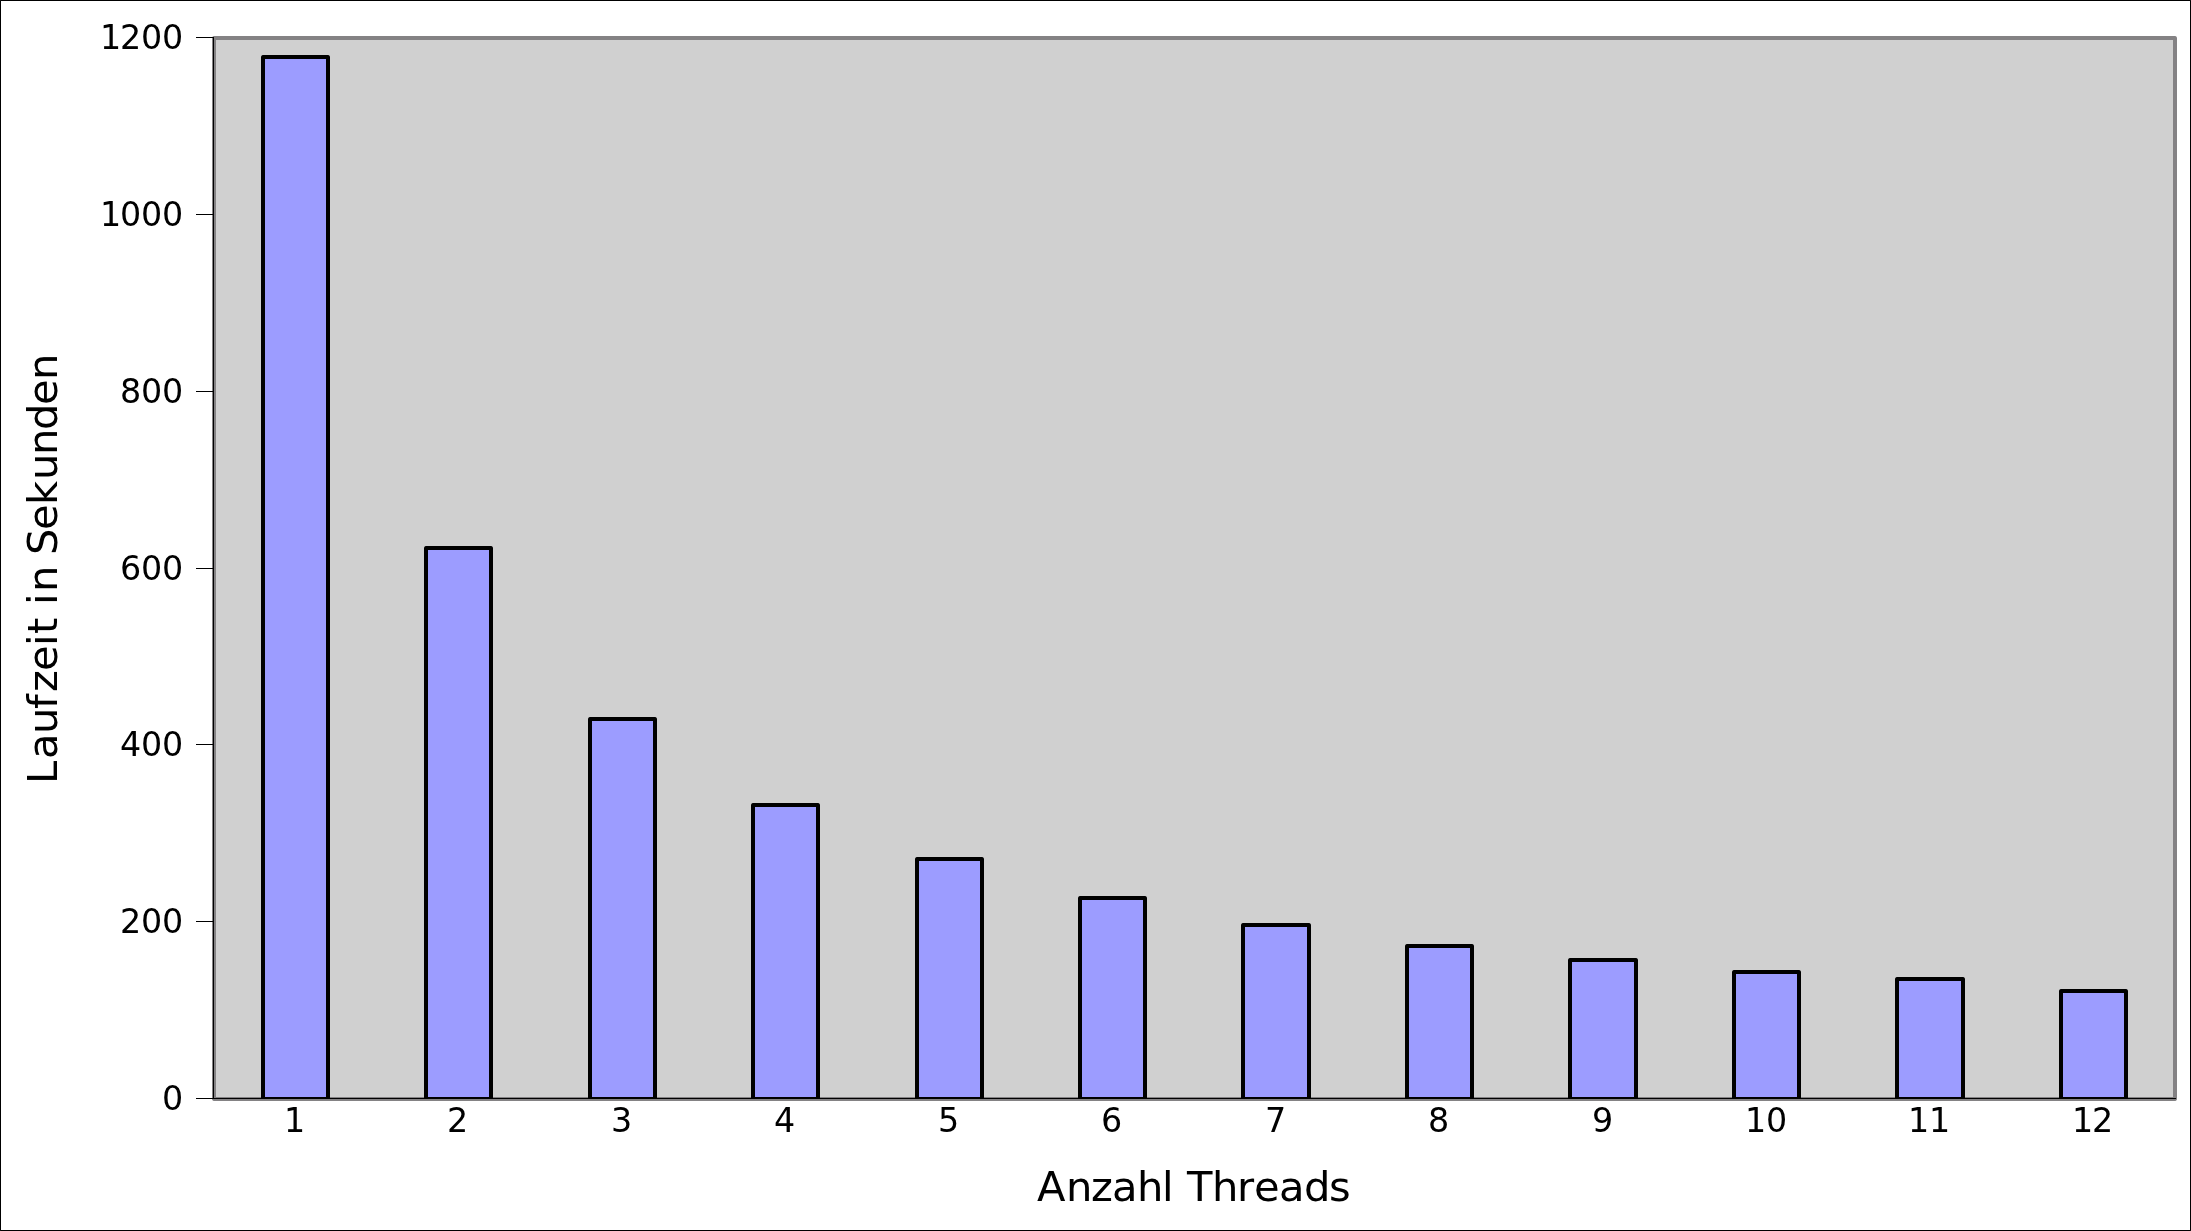
\includegraphics[height=7cm]{/home/christian/Uni/5_Semester/HR/HR-1213/Blatt4/leistungsgraph.png}
\caption{\textbf{Laufzeitmessung für verschiedene Threadzahlen.} \\512 Interlines, 1024 Iterationen, Messwerte jeweils in Sekunden}
\end{figure}

\begin{table}[!h]
\begin{tabular}{|l|r|r|r|r|r|}
\hline
Interlines&1. Messung&2. Messung&3. Messung&Mittel\\
\hline
1&	0,0084	&0,0079	&0,0092	&0,0085\\
2&	0,0120	&0,0124	&0,0115	&0,0120\\
4&	0,0197	&0,0184	&0,0203	&0,0194\\
8&	0,0673	&0,0450	&0,0553	&0,0559\\
16&	0,1353	&0,1673	&0,1755	&0,1594\\
32&	0,5009	&0,5733	&0,6675	&0,5806\\
64&	1,9164	&2,3005	&2,5123	&2,2430\\
128&	7,6345	&7,6356	&9,7240	&8,3314\\
256&	30,7198	&33,1656	&37,9655	&33,9503\\
512&	121,6844	&122,5537	&131,9247	&125,3876\\
1024&	486,2178	&488,4605	&545,6306	&506,7696\\

\hline
\end{tabular}
\caption{\textbf{Laufzeitmessung für verschiedene Interlinezahlen.} \\12 Threads, 1024 Iterationen, Messwerte jeweils in Sekunden}
\end{table}
\end{document}
